\documentclass[english]{article}
\usepackage{amsmath}
\usepackage{graphicx}

\usepackage[draft]{fixme}
\usepackage{babel}

\newcommand{\+}[1]{\ensuremath{\boldsymbol{\mathrm{#1}}}}

\begin{document}


\begin{figure}
\centering
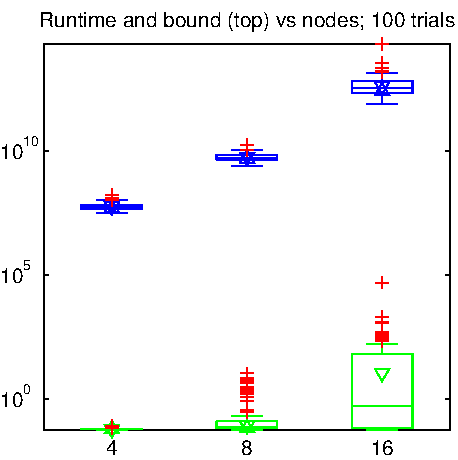
\includegraphics[width=0.49\linewidth, clip]{nodes_time}
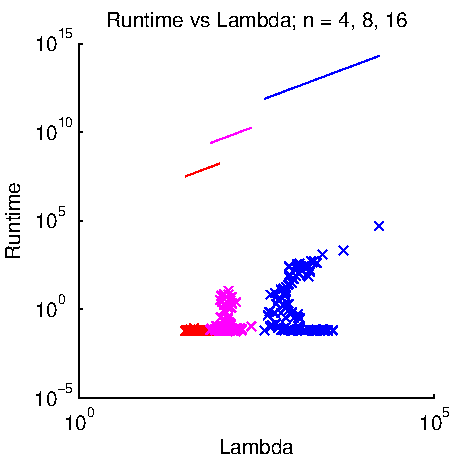
\includegraphics[width=0.49\linewidth, clip]{lambda_time}
\caption{Actual runtime and theoretical bound  \emph{Left:} Scaling with respect to problem size. Each box plot represents 100 trials; top (blue) are theoretical bounds and bottom (green) are actual runtimes. \emph{Right:} Scaling with respect to curvature $\Lambda$. Solid line is theoretical bound, and scatter points are actual runtimes. Red, magenta, blue and 4, 8, 16 nodes respectively.} \label{fig:time}
\end{figure}
\section{Experiments}
\begin{figure}
\centering
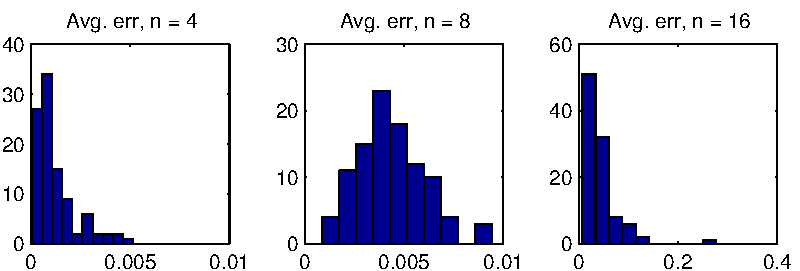
\includegraphics[width=\linewidth, clip]{errors}
\caption{Average 1-norm deviations from truth (according to Junction Tree) in singleton marginals. Plot of 100 trials per size.} \label{fig:errors}
\end{figure}

We generated 100 complete graphs for $N = 4,8,16$ nodes, drawing each $\theta_i$ uniformly from $[-2,2]$, $W_{ij}$ uniformly from $[0, 1]$ and applying the de-biasing procedure in Section \fxwarning{Reference!}. We set $\varepsilon = 0.01$. As shown in Figure~\ref{fig:time}, our empirical worst-case results do indeed follow the shape of our theoretical bound, as a function of both problem size and curvature $\Lambda$. This suggests that the bound is in practice tight. In addition, as shown in Figure~\ref{fig:errors} the total 1-norm error of the singleton marginals remain low, even with our relatively course tolerance on the free energy term.

\end{document}
